%!TEX root = ../thesis.tex
\section{Methodology}\label{sec:methodology}
This section describes all strategies and concepts \drivebuild{} follows to formalize test cases and to implement a test life cycle.
It also explains the cycle of the runtime verification process and the underlying strategies concerning the communication between the components of \drivebuild{} and the communication between \drivebuild{} and clients.

\subsection{Test Case Formalization}
The test case formalization specifies a test environment, the behavior of participants, the test criteria and the data which either \glspl{av} under test require or which has to be collected \eg{} for training data.
Since there are many different kinds of \glspl{adas} which simulation based testing can validate the formalization concentrates on a subset of \glspl{adas}.
To determine a subset of \glspl{adas} which implement essential functionality of \glspl{av} and are safety critical I read many recent papers that discuss \glspl{adas}.
\Cref{tab:targetAdas} lists the targeted \glspl{adas} and groups them by their function.
\begin{table}
    \centering
    \caption{%
        Target \glspl{adas} --- Lists all \glspl{adas} that the formalization aims to support.
        The \glspl{adas} are grouped based on their functionality and thus by the metrics they require to work.
    }\label{tab:targetAdas}
    \medskip
    %!TEX root = ../thesis.tex
\def\tabularxcolumn#1{m{#1}}
\begin{tabularx}{\linewidth}{c l X}
    \toprule
    \bfseries Group & \bfseries Supported \glspl{adas} & \bfseries Description \\
    \midrule
    1 & \makecell[l]{%
        Collision avoidance system\\
        Forward Collision Warning\\
        Emergency Brake Assist\\
        Intersection assistant\\
        Turning assistant
    } & Systems that avoid or reduce the severity of collisions or at least warn a driver about them\\
    \midrule
    2 & \makecell[l]{%
        Intelligent speed adaptation\\
        Cruise control\\
        Adaptive cruise control\\
        Active Brake Assist
    } & Systems that control the speed of an \gls{av} or keep a safe distance to other participants\\
    \midrule
    3 & \makecell[l]{%
        Lane centering\\
        Lane departure warning system\\
        Lane change assistance\\
        Wrong-way driving warning
    } & Systems that observe the relative position of an \gls{av} on a lane or determine the direction of a lane.\\
    \bottomrule
\end{tabularx}


\end{table}
Hence \glspl{adas} in same the group presumably share the same minimum set of metrics which they require to operate.
For each group \cref{tab:reqData} identifies which basic metrics they require.
\begin{table}
    \caption{%
        Minimum required metrics --- Lists the minimal set of metrics which \glspl{adas} in the same group (see \cref{tab:targetAdas}) presumably require.
    }\label{tab:reqData}
    \medskip
    %!TEX root = ../thesis.tex
\def\tabularxcolumn#1{m{#1}}
\begin{tabularx}{\linewidth}{X c c c}
    \toprule
    \bfseries Type of data                       & \bfseries Group 1 & \bfseries Group 2 & \bfseries Group 3 \\
    \midrule
    Distance to other traffic participants       & \checkmark{}      & \checkmark{}      & \ding{53}         \\
    Distance to lane markings and road edges     & \ding{53}         & \ding{53}         & \checkmark{}      \\
    Angle of \gls{av} to the road                & \ding{53}         & \checkmark{}      & \ding{53}         \\
    Speed                                        & \checkmark{}      & \checkmark{}      & \ding{53}         \\
    Relative speed to other traffic participants & \checkmark{}      & \checkmark{}      & \checkmark{}      \\
    \bottomrule
\end{tabularx}


\end{table}
It reveals that some groups of \glspl{adas} require more metrics like Group~2 and others require only a few metrics like Group~3.
All considered metrics result from the basic data types position of \gls{av}, position of lane markings and speed.
To test an \gls{av} which integrates \glspl{adas} of these groups the \gls{av} requires the appropriate metrics either directly or in the form of other data types \eg{} camera or \gls{lidar} images which the underlying \gls{ai} uses to extract the required metrics itself.
Hence it is not sufficient for the formalization to provide only metrics which \glspl{adas} require directly but also to provide other common data types.\\
The formalization in this work describes test cases declaratively which avoids any need to compile or interpret the formalized test case.
Further the formalization is based on \gls{xml} which allows to define a \gls{xsd} which can validate a test case to make sure that it is specified properly before it is processed.
Additionally \gls{xml} has great support in many languages and is well-known for decades.
The formalization follows a modular approach in that separates the \glspl{dbe} which describe the static environments from \glspl{dbc} which describe participants and the test criteria.
This separation allows to reuse environments throughout multiple scenarios and avoids duplication of possible very complex environments.
\subsubsection{Formalization of Environments}
An environment is a two dimensional world.
The coordinate system defines positions with a x- and y-axis which have the unit meters and specifies rotation in anti clockwise manner starting with \ang{0} pointing in positive x direction as shown in \cref{fig:envCooSystem}.
This representation sticks to commonly used mathematical representations and thus avoids additional translations between models and the formalization.
\begin{figure}
    \centering
    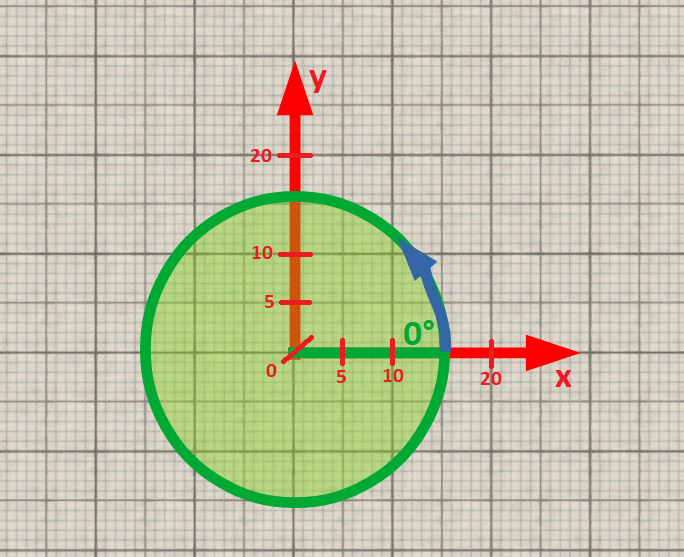
\includegraphics[width=.6\linewidth]{pictures/2019-08-12_envCooSystem.png} % chktex 8
    \medskip
    \caption{%
        Environment coordinate system --- Visualizes the theoretical view on an environment.
        For purpose of illustration the underlying grid shows squares which group 5 by 5 cells where each cell has an edge length of \SI{1}{\metre}.
        This grid is not visible during a simulation.
    }\label{fig:envCooSystem}
\end{figure}
A \gls{dbe} specifies environment elements \ie{} roads and obstacles.
A road has a course, a number of left and right lanes and optionally has road markings and a name.
The course is a sequence of tuples where each tuple contains a road center point and the current width of the road at that point.
This representation allows to easily calculate the distance of an \gls{av} to the road center and to determine the direction of lanes.
The number of left and right lanes influences the types of road markings in case a road has markings.
Right lanes go in the same direction as the sequence of the road center points.
Left lanes go in the opposite direction.
In order to define basic static surroundings like buildings the formalization allows obstacles of type cube, cylinder, cone and bump.
Obstacles can not be moved by participants, do not deform and are unbreakable.
\Cref{fig:exampleEnvironmentVis} depicts simple examples of generated environment elements.
\begin{figure}
    \centering
    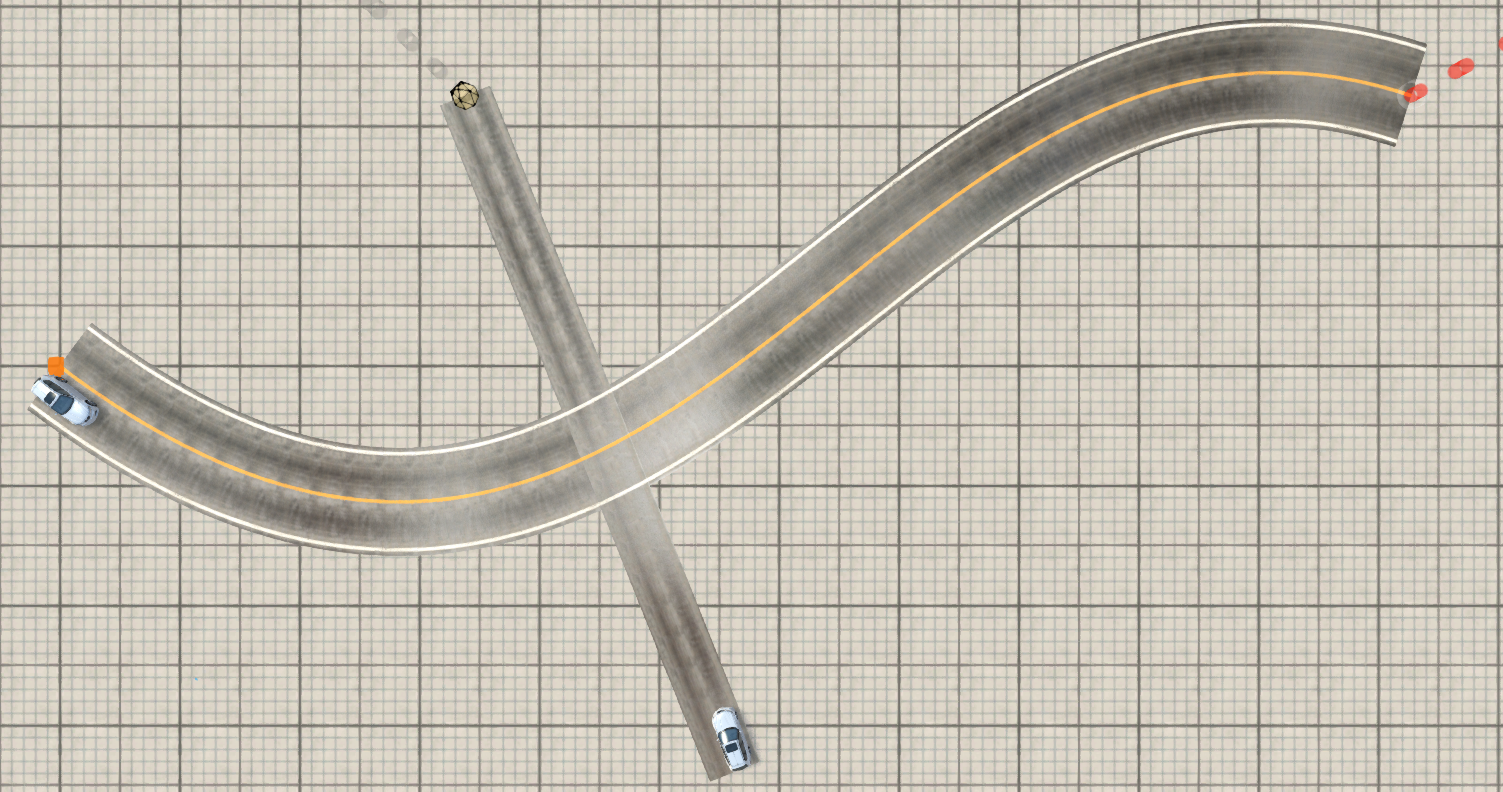
\includegraphics[width=\linewidth]{pictures/2019-08-15_simpleLanes.png} % chktex 8
    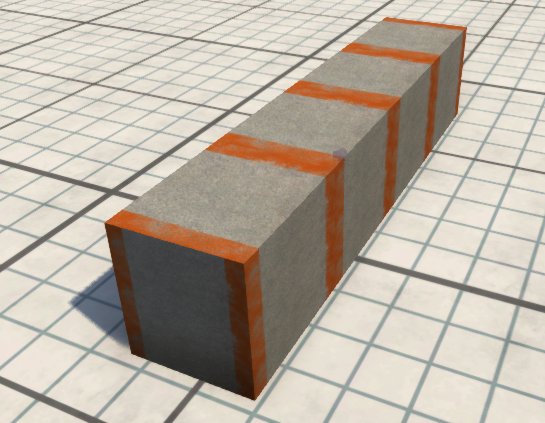
\includegraphics[height=70px]{pictures/cube.png}
    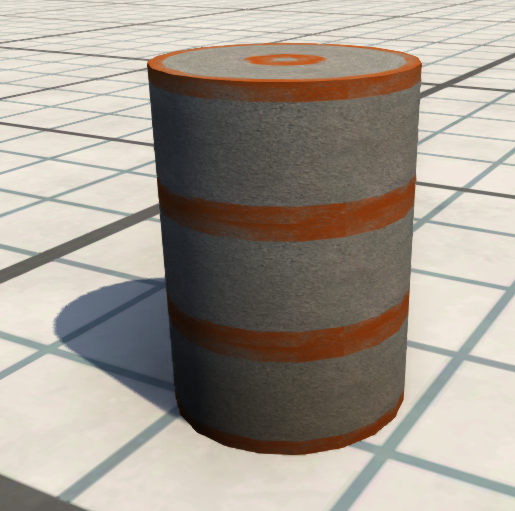
\includegraphics[height=70px]{pictures/cylinder.png}
    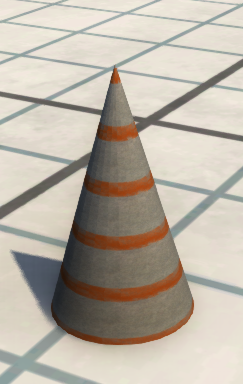
\includegraphics[height=70px]{pictures/cone.png}
    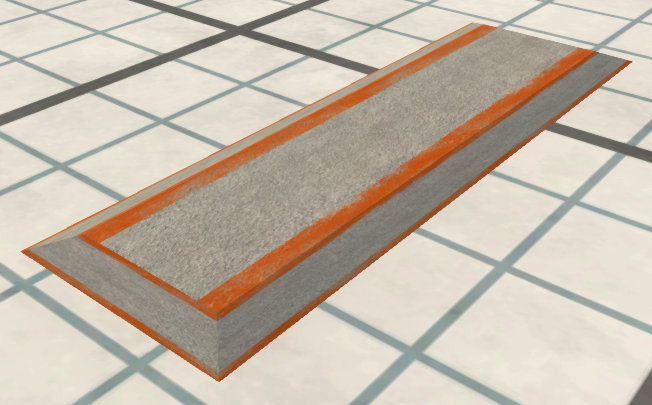
\includegraphics[height=70px]{pictures/bump.png}
    \medskip
    \caption{%
        Visualization of example environment elements --- Shows generated static environment elements including two roads and multiple obstacles.
        For purpose of illustration the underlying grid shows squares which group 5 by 5 cells where each cell has an edge length of \SI{1}{\metre}.
        This grid is not visible during a simulation.
        \Cref{fig:exampleEnvironment,fig:exampleObstacleDefinitions} in the appendix show the declarations to generate these environment elements.
    }\label{fig:exampleEnvironmentVis}
\end{figure}
\subsubsection{Formalization of Criteria}
The test criteria divide in precondition, success and fail criteria.
Typically a test is considered as successful if it ends without triggering the fail criterion.
In the context of testing \glspl{av} this may not be always true since the tests are very complex and there are cases where an \gls{av} does not succeed but a tester does not want the test to be marked as failed.
A very common example is a test like \enquote{The \gls{av} is successful if it reaches a certain position and fails if it takes any damage or goes off-road}.
If the \gls{av} under test does not move at all it does not pass the test.
That the \gls{av} does currently not move does not imply that is not going to move at some point in the future.
Hence it can not be concluded that the test failed.
To describe such results \drivebuild{} uses a three-valued logics.
The most basic one is the Kleene and Priest logics~\cite{kleeneLogics} which declares besides \iltrue{} and \ilfalse{} also the value \ilunknown{}.
Since the third value \ilunknown{} is neutral to all connectives it can express that a criterion could not be determined or is currently not considered without influencing the outcome of the overall criterion.
The definition of test criteria follows the concept of temporal logic and thus defines \glspl{sc}, \glspl{vc} and connectives (\iland{}, \ilor{} and \ilnot{}) which can be nested as \cref{fig:nesting} visualizes.
\begin{figure}
    \centering
    \begin{tikzpicture}[%
        ->,
        >=stealth
    ]
    \node (evaluation) {\itshape criterion};
    \node[above=of evaluation] (start) {};
    \node[below=of evaluation] (criterion) {\itshape evaluation};
    \node[left=of criterion] (connective) {\itshape connective};
    \node[below=of connective] (and) {and};
    \node[right=of and] (or) {or};
    \node[left=of and] (not) {not};
    \node[below=of criterion] (sc) {\glstext{sc}};
    \node[right=of sc] (vc) {\glstext{vc}};

    \path
        (start) edge (evaluation)
        (evaluation) edge (criterion)
        (evaluation) edge[bend left]  (connective)
        (connective) edge[bend left] (evaluation)
        (criterion) edge (sc)
        (criterion) edge (vc)
        (vc) edge[bend right] (evaluation)
        (connective) edge (not)
        (connective) edge (and)
        (connective) edge (or);
\end{tikzpicture}


    \medskip
    \caption{%
        Nesting of a criterion --- Shows the allowed nesting structure for \glspl{sc}, \glspl{vc} and connectives to define a criterion. Italic types are abstract.
    }\label{fig:nesting}
\end{figure}
\Glspl{sc} as well as \glspl{vc} evaluate the current state of the simulation or an \gls{av} and determine whether it fulfills a certain condition.
\Glspl{sc} yield in case the criterion can be evaluated either \iltrue{} or \ilfalse{}.
Otherwise it returns \ilunknown{}.
\Glspl{vc} restrict whether the inner criterion has to be considered in the evaluation of the parent criterion.
If the condition of the \gls{vc} is \iltrue{} the inner criterion is evaluated and the \gls{vc} returns its result.
Otherwise the \gls{vc} returns \ilunknown{}.
The introduction of \glspl{vc} allows to evaluate different criteria under different circumstances.
This allows to enable or disable criteria under certain circumstances.
\Eg{} define a fail criterion like \enquote{While \gls{av} \(A\) drives on road \(R\) it must not exceed a speed limit of \(S\)}.
In this case the speed of \(A\) should only be evaluated as long as \(A\) drives on \(R\) and return ideally either \iltrue{} or \ilfalse{}.
If \(A\) is not on \(R\) \ilunknown{} shall be returned to ignore the criterion.
Another use case for \glspl{vc} may be to define that an \gls{av} is allowed to leave the road as long as it is in a certain area \eg{} to avoid an obstacle or another participant that blocks the road in this area.
\Cref{tab:criteriaTypes} lists all supported kinds of criteria and whether they can be used as \gls{vc} or \gls{sc}.
\begin{table}
    \centering
    \caption{%
        Test criteria --- Lists all supported test criteria, describes their purpose and characterizes whether these can be used for \glspl{vc} or \glspl{sc}.
    }\label{tab:criteriaTypes}
    \medskip
    %!TEX root = ../thesis.tex
\begin{tabularx}{\linewidth}{l X c c}
    \toprule
    \bfseries Type & \bfseries Description & \bfseries \glstext{vc} & \bfseries \glstext{sc} \\
    \midrule
    position & Checks whether an \gls{av} is at a certain position or within a certain radius of it & \checkmark{} & \checkmark{} \\
    area & Checks whether an \gls{av} is within a certain area & \checkmark{} & \checkmark{} \\
    lane & Checks whether an \gls{av} drives on a certain lane or off-road & \checkmark{} & \checkmark{} \\
    speed & Checks whether the speed of an \gls{av} is below a given velocity & \checkmark{} & \checkmark{} \\
    damage & Checks whether an \glspl{av} is damaged & \checkmark{} & \checkmark{} \\
    time & Checks whether the simulation is currently within a certain interval of ticks & \checkmark{} & \ding{53} \\
    distance & Checks whether the distance between two \glspl{av} or between an \gls{av} and the center of the lane driving on is smaller than a given distance & \checkmark{} & \checkmark{} \\
    \glstext{ttc} & Checks whether the \glsfirst{ttc} of an \gls{av} and another participant or obstacle is smaller than a given value & \checkmark{} & \ding{53} \\
    \bottomrule
\end{tabularx}


\end{table}
\Cref{fig:exampleCriteria} in the appendix shows example definitions for all of them.
Using the mechanism which \cref{sec:runtimeVerification} explains a tester can introduce additional client side criteria.
\subsubsection{Formalization of Participants}
The declaration of a participant specifies always a car model and an initial state.
The chosen model fixes the shape and the physics of the participant.
The set of available models is a predefined set which comes with \beamng{}.
The initial state specifies the initial position and the initial orientation of a participant.
If a participant is an \gls{av} the underlying \gls{ai} and its \glspl{adas} require data to operate.
The formalization allows to declaratively specify this data which a simulation has to collect and provide.\\
Resulting from the metrics which \glspl{adas} require in \cref{tab:reqData} and the available test criteria in \cref{tab:criteriaTypes} I determined multiple types of request data (see \cref{tab:aiData}) which a formalization can declare and which a simulation can provide.
\begin{table}
    \caption{%
        Available request data --- Lists all types of request data which an \gls{ai} that registered at a simulation can possibly request and whether it can be considered as sensor data.
    }\label{tab:aiData}
    \medskip
    %!TEX root = ../thesis.tex
\begin{tabularx}{\linewidth}{l X c}
    \toprule
    \bfseries Type          & \bfseries Description                                                             & \bfseries Sensor Data \\
    \midrule
    position                & Absolute position of an \gls{av}                                                  & \ding{53}             \\
    speed                   & Absolute speed of an \gls{av}                                                     & \checkmark{}          \\
    steering angle          & Current steering angle of the steering wheel                                      & \checkmark{}          \\
    \Glstext{lidar}         & Distance data provided by a \gls{lidar} sensor                                    & \checkmark{}          \\
    camera                  & Camera images either colored, annotated or with depth information                 & \checkmark{}          \\
    damage                  & Detects whether an \gls{av} is damaged                                            & \checkmark{}          \\
    distance to road center & Distance to the center of the nearest road                                        & \ding{53}             \\
    heading angle           & Angle between the orientation of a participant and the center of the nearest road & \ding{53}             \\
    bounding box            & The bounding box of a participant                                                 & \ding{53}             \\
    road edges              & Sequences of points for the right and left edge of a road                         & \ding{53}             \\
    \bottomrule
\end{tabularx}


\end{table}
It also shows which of the request data can be considered as sensor data and thus marks on which request data an \gls{ai} should rely in order to be realistic.
The other types of request data can be used to collect training data, to compare the computed results of an \gls{ai} to a ground truth or to implement additional client side criteria before or after the computations which an \gls{ai} does.\\
In case the participant is not autonomous the declaration may specify a movement.
A movement is a sequence of waypoints which a participant has to follow.
A waypoint is a position at which the behavior of a participant may change.
It also has a tolerance value which avoids that a participant has to precisely reach a position and allows to pass by in a certain distance.
A waypoint optionally defines a speed limit or a target speed which a participant has to obey until it reaches the next waypoint that specifies another value for them.
Both the initial state and all waypoints have an attribute which specifying the current movement mode of a participant.
The movement mode is one of \mmmanual{}, \mmautonomous{} and \mmtraining{}.
If the current movement mode of a participant is \mmmanual{} the car heads straight to the next waypoint and the target speed as well as the speed limit apply.
If the movement mode is \mmautonomous{} the simulation requests the \gls{ai} that registered for controlling the \gls{av} frequently and provides it with data.
If the movement mode is set to \mmtraining{} the \gls{av} acts the same way it does in \mmmanual{} but the simulation requests the connected \gls{ai} like in \mmautonomous{}.
In contrast to \mmautonomous{} the \gls{ai} can not control the \gls{av}.
However, the \gls{ai} can still control the simulation.
This mode is geared towards collecting training data for \glspl{ai}.
The strategy to allow to change movement modes at each waypoint enables to mix sections where a participant is forced to follow a path, where an \gls{ai} has to control it or where to collect data.
\Cref{fig:exampleParticipant,fig:exampleAIDataRequests} in the appendix show example definitions of participants as well as example declarations of many request data.
\Cref{fig:exampleParticipantVis} shows the corresponding graphical representation of the participant and its movement.
\begin{figure}
    \centering
    \includegraphics[width=.9\linewidth]{pictures/2019-08-15_ParticipantMovements.png} % chktex 8
    \medskip
    \caption{%
        Visualization of example participants --- Shows participants and their movements generated from the declarations in \cref{fig:exampleParticipant} in the appendix.
        The green line marks the parts of a path where a participant is in \mmmanual{} mode and has to follow the waypoints.
        The red stripe marks the area an \gls{av} in \mmautonomous{} mode is expected to follow but not forced to.
        In this case the participants do not change their movement mode during the simulation.
    }\label{fig:exampleParticipantVis}
\end{figure}

\subsection{Test Life Cycle}\label{sec:testCycle}
\Cref{fig:testCycle} shows all phases of the test life cycle and groups them into the four main steps \textcolor{blue}{input validation}, \textcolor{magenta}{extraction}, \textcolor{cyan}{transformation} and \textcolor{red}{execution}.\\
\begin{figure}
    \centering
    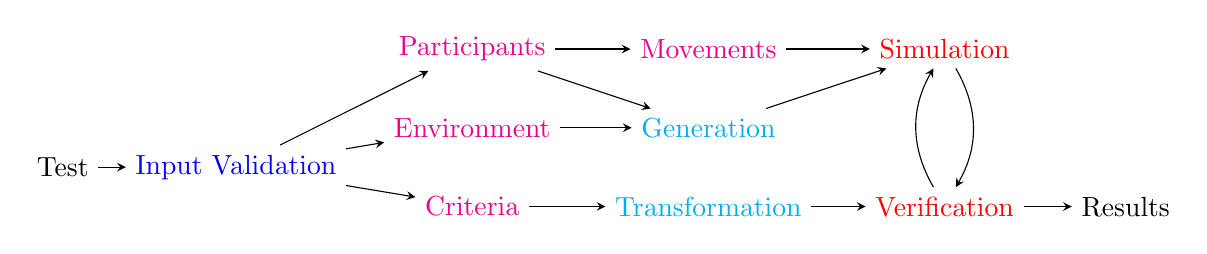
\begin{tikzpicture}[%
        ->,
        >=stealth
    ]
    \node at (-3.2,0) (Tester) {Test};
    \node at (-1,0) (Validation) {\textcolor{blue}{Input Validation}};
    \node at (2,0.5) (Environment) {\textcolor{magenta}{Environment}};
    \node at (2,1.5) (Participants) {\textcolor{magenta}{Participants}};
    \node at (5,1.5) (Movements) {\textcolor{magenta}{Movements}};
    \node at (2,-0.5) (Criteria) {\textcolor{magenta}{Criteria}};
    \node at (5,-0.5) (Transform) {\textcolor{cyan}{Transformation}};
    \node at (5,0.5) (Generation) {\textcolor{cyan}{Generation}};
    \node at (8,1.5) (Simulation) {\textcolor{red}{Simulation}};
    \node at (8,-0.5) (Verification) {\textcolor{red}{Verification}};
    \node at (10.3,-0.5) (Results) {Results};
    \path
        (Tester) edge (Validation)
        (Validation) edge (Environment)
        (Environment) edge (Generation)
        (Generation) edge (Simulation)
        (Validation) edge (Participants)
        (Participants) edge (Movements)
        (Movements) edge (Simulation)
        (Participants) edge (Generation)
        (Validation) edge (Criteria)
        (Criteria) edge (Transform)
        (Transform) edge (Verification)
        (Verification) edge[bend left] (Simulation)
        (Simulation) edge[bend left] (Verification)
        (Verification) edge (Results);
\end{tikzpicture}

    \medskip
    \caption{%
        Test life cycle --- Visualizes the four main steps of processing a formalized test.
        The input validation step is \textcolor{blue}{blue}, the extraction step is \textcolor{magenta}{magenta}, the transformation step is \textcolor{cyan}{cyan} and the execution step is \textcolor{red}{red}.
    }\label{fig:testCycle}
\end{figure}
The input validation checks whether the test case is broken or malformed and validates it against the \gls{xsd} which enforces the structure of the formalized test case.
If the test case is valid the process extracts the environment description, the test criteria and the participants.
It passes the information about roads, obstacles and participants in the environment to the generator which creates representations that are compatible with the underlying simulator.
The representation of the movements of the participants are passed directly to \beamng{} which applies them sequentially to the appropriate participants as soon as the simulation started.
The transformation step creates Kleene and Priest logics expressions which represent the defined test criteria.
The verification process uses these expressions to verify the criteria during the simulation.
Then \beamng{} starts the execution of the test and sets up the runtime verification process (see \cref{sec:runtimeVerification}).
As soon as the runtime verification is able to determine whether the test succeeded or failed it stops the simulation and returns its test result.

\subsection{Runtime Verification}\label{sec:runtimeVerification}
The runtime verification cycle applies synchronous simulation (see \cref{sec:background}) and \cref{fig:runtimeVerification} depicts its five phases.
\begin{figure}
    \centering
    \smartdiagram[flow diagram:horizontal]{%
        Verify criteria, Request \glspl{ai}, Control, Step, Pause
    }
    \medskip
    \caption{%
        Runtime verification cycle --- Depicts the main phases which implement the runtime verification and applies the synchronous simulation.
    }\label{fig:runtimeVerification}
\end{figure}
The first phase checks whether the current state of the simulation yields a test result.
Therefore it uses a decision tree where the leaves represent test results and the inner nodes represent the evaluation of the precondition, the fail and the success criterion.
The inner nodes work with lazy evaluation and \cref{fig:verificationDecision} shows the complete tree.
\begin{figure}
    \centering
    \begin{tikzpicture}[%
    ->,
    >=stealth
]
    \node (start) {};
    \node[right=of start] (preconds) {Precondition};
    % \node[below=of preconds] (skipped) {\underline{\vsmskipped{}}}; % FIXME Does not work
    \node[below=of preconds] (skipped) {\underline{\code{SKIPPED}}};
    \node[right=of preconds] (fail) {Fail criterion};
    % \node[below=of fail] (tcFail) {\underline{\vsmfailed{}}}; % FIXME Does not work
    \node[below=of fail] (tcFail) {\underline{\code{FAILED}}};
    \node[right=of fail] (success) {Success criterion};
    % \node[below=of success] (tcSuccess) {\underline{\vsmsucceeded{}}}; % FIXME Does not work
    \node[below=of success] (tcSuccess) {\underline{\code{SUCCEEDED}}};
    % \node[right=of success] (undetermined) {\underline{\vsmunknown{}}}; % FIXME Does not work
    \node[right=of success] (undetermined) {\underline{\code{UNKNOWN}}};

    \path (start) edge (preconds);
    \draw[red] (preconds) edge (skipped);
    \draw[green] (preconds) edge[bend left] (fail);
    \draw[blue] (preconds) edge[bend right] (fail);
    \draw[green] (fail) edge (tcFail);
    \draw[red] (fail) edge[bend left] (success);
    \draw[blue] (fail) edge[bend right] (success);
    \draw[green] (success) edge (tcSuccess);
    \draw[red] (success) edge[bend left] (undetermined);
    \draw[blue] (success) edge[bend right] (undetermined);
\end{tikzpicture}

    \medskip
    \caption{%
        Test result decision tree --- Visualizes the structure of the decision tree which determines the current test result.
        Underlined nodes are leaves and represent test results.
        The inner nodes represent the criteria of the test.
        Arrows describe the transitions from node to node which depends on whether a criterion evaluated to \colorbox{green!50}{true}, \colorbox{red!50}{false} or \colorbox{blue!40}{unknown}.
    }\label{fig:verificationDecision}
\end{figure}
If the decision tree yields either \trskipped{}, \trfailed{} or \trsucceeded{} the simulation stops and returns the current test result as final test result.
In this case all \glspl{ai} which are registered at the simulation are notified about the end of the simulation as well.
If the current test result is \trunknown{} the runtime verification cycle continues with the next phase.
The second phase implements the exchange of data with \glspl{ai}.
Therefore it updates all data of any sensor and all properties of any participant which were declared in the \gls{dbc} or are required to evaluate the test criteria.
The phase also searches for all \glspl{av} that are in movement mode \mmautonomous{} or \mmtraining{}, notifies the \glspl{ai} which registered for these \glspl{av} about the availability of new data and waits for them to send commands which control the \glspl{av} or the simulation.
\Cref{fig:aiSimProtocol} depicts the three-way protocol which the communication uses.
\begin{figure}
    \centering
    \documentclass{standalone}

\usepackage[acronym,automake,toc]{glossaries}
\usepackage{pgf-umlsd}

\makeglossaries%
\loadglsentries{../acronyms.tex}

\begin{document}

\begin{sequencediagram}
    \newthread{sim}{:Simulation}
    \newinst{dummy}{Dummy placeholder}
    \newthread{ai}{:\glstext{ai}}
    \begin{call}{ai}{Wait for request}{sim}{Send alive message}
        \begin{callself}{sim}{Simulate}{}
        \end{callself}
    \end{call}
    \begin{call}{ai}{Request simulation data}{sim}{Send simulation data}
    \end{call}
    \begin{callself}{ai}{Calculate control commands}{}
    \end{callself}
    \begin{call}{ai}{Control simulation}{sim}{Send alive message}
    \end{call}
\end{sequencediagram}


\end{document}

    \medskip
    \caption{%
        Communication between a simulation and an \glstext{ai} --- Visualizes the messages of the three-way protocol sent for exchanging data between a simulation and an \glstext{ai}.
    }\label{fig:aiSimProtocol}
\end{figure}
The first message registers an \gls{ai} at a certain simulation for a certain \gls{av} and blocks until the simulation notifies it about new data.
Its response contains the current state of the simulation which is either \ssrunning{}, \ssfinished{}, \sscanceled{} or \sstimeout{}.
The state of the simulation may be \ssunknown{} which is only the case if the simulation could not be found.
These states allow an \gls{ai} to determine whether a simulation exists and whether it still runs or already stopped.
They also allow to determine the reason why the simulation stopped.
If the state of the simulation is \ssrunning{} the \gls{ai} requests sensor data or properties of its associated \gls{av} for which it needs to calculate control commands.
A control command for an \gls{av} is a tuple which contains values for acceleration, brake intensity and steering angle.
A command to control a simulation contains only the test result which has to be enforced.
The opportunity to control a simulation allows an \gls{ai} to eventually stop the simulation after the evaluation of client side criteria.\\
The control phase applies the commands which the \glspl{ai} sent.
In case one of them enforces a test result the simulation stops.
Otherwise the phase applies all control commands of the \glspl{ai} to their associated \gls{av} the runtime verification continues with the next phase.
In this phase \beamng{} calculates the changes to the simulation for the next number of ticks as defined by the \gls{ai} frequency, applies them and pauses the simulation again.
Then the runtime verification cycle starts from the beginning.

\subsection{Cluster Architecture}
The architecture of \drivebuild{} uses a master slave model.
The slave components are \glspl{simnode} that manage running simulations and runtime verification processes.
The master component is the \gls{mainapp}.
It organizes all \glspl{simnode} and offers the entry point for all clients and \glspl{ai}.\\
\Cref{fig:systemArch} depicts all logical components of \drivebuild{}, their data flow and how they are grouped to modules that can be distributed over a cluster.
\begin{figure}
    \centering
    %!TEX root = ../thesis.tex
\begin{tikzpicture}[%
    ->,
    >=stealth
]
\tikzset{%
    node distance=2.5
}
\node (tester) {Tester};
\node[below=of tester] (tcmanager) {\Glstext{tcmanager}};
\node[right=of tester] (ai) {\Glstext{ai}};
\node[below=of ai] (communicator) {{{\scshape Communicator}}};
\node[below=4 of tcmanager] (simcontroller) {\Glstext{simcontroller}};
\node[left=1.3 of simcontroller] (transformer) {{{\scshape Transformer}}};
\node[above=.1 of transformer] (fitExtension) {};
\node[left=1.9 of transformer] (generator) {{{\scshape Generator}}};
\node[above=1.8 of transformer] (dbms) {\Glstext{dbms}};
\node[above=1.7 of dbms] (stats) {\Glstext{statsmanager}};
\node[above=of stats] (researcher) {Researcher};
\node[below=of transformer] (kptransformer) {\Glstext{kptransformer}};
\node[below=of simcontroller] (verificator) {\mltn{Runtime Verification\\Process 1\ldots N}};
\node[right=0.5 of verificator] (simulatorA) {Simulation 1\ldots N};

% Client backgrounds
\node[zlayer=back,fill=clusterClient,fit={(researcher)}] {};
\node[zlayer=back,fill=clusterClient,fit={(tester)}] {};
\node[zlayer=back,fill=clusterClient,fit={(ai)}] {};
% Stack 1
\node[below right=-0.5mm and 0.5mm of ai.south west] (aiStackA) {};
\node[below right=-0.5mm and -0.5mm of ai.south east] (aiStackB) {};
\node[below right=0.5mm and -0.5mm of ai.north east] (aiStackC) {};
\node[zlayer=back,fill={rgb,255:red,112;green,112;blue,255},fit={(aiStackA)(aiStackB)(aiStackC)},inner sep=0] (aiStackA) {};
% Stack 2
\node[below right=-1.5mm and 0.5mm of aiStackA.south west] (aiStackAA) {};
\node[below right=-1.5mm and -1.5mm of aiStackA.south east] (aiStackBB) {};
\node[below right=0.5mm and -1.5mm of aiStackA.north east] (aiStackCC) {};
\node[zlayer=back,fill={rgb,255:red,0;green,0;blue,255},fit={(aiStackAA)(aiStackBB)(aiStackCC)},inner sep=0] {};
% Redraw previous stacks in reverse order
\node[zlayer=back,fill={rgb,255:red,112;green,112;blue,255},fit={(aiStackA)(aiStackB)(aiStackC)},inner sep=0] (aiStackA) {};
\node[zlayer=back,fill=clusterClient,fit={(ai)}] {};

% SimNode backgrounds
\node[zlayer=back,fill=clusterSimNode,fit={(simulatorA)(kptransformer)(verificator)(generator)(fitExtension)}] (server) {};
% Stack 1
\node[below right=0mm and 3mm of server.south west] (simNodeStackA) {};
\node[below right=0mm and 0mm of server.south east] (simNodeStackB) {};
\node[below right=3mm and 0mm of server.north east] (simNodeStackC) {};
\node[zlayer=back,fill={rgb,255:red,112;green,255;blue,112},fit={(simNodeStackA)(simNodeStackB)(simNodeStackC)},inner sep=0] (stackA) {};
% Stack 2
\node[below right=0mm and 3mm of stackA.south west] (simNodeStackAA) {};
\node[below right=0mm and 0mm of stackA.south east] (simNodeStackBB) {};
\node[below right=3mm and 0mm of stackA.north east] (simNodeStackCC) {};
\node[zlayer=back,fill={rgb,255:red,0;green,220;blue,0},fit={(simNodeStackAA)(simNodeStackBB)(simNodeStackCC)},inner sep=0] {};
% Redraw previous stacks in reverse order
\node[zlayer=back,fill={rgb,255:red,112;green,255;blue,112},fit={(simNodeStackA)(simNodeStackB)(simNodeStackC)},inner sep=0] (stackA) {};
\node[zlayer=back,fill=clusterSimNode,fit={(simulatorA)(kptransformer)(verificator)(generator)(fitExtension)}] (serverRedraw) {};

% MainApp background
\node[zlayer=back,fill=clusterMicroService,fit={(tcmanager)(communicator)(stats)}] (microserviceA) {};

% DBMS background
\node[zlayer=back,fill=clusterDbms,fit={(dbms)}] (dbmsComponent) {};

\path
    (tester) edge node[above]{SimulationID} node[below]{VehicleID} (ai)
    (tester) edge[bend right] node[rotate=90,above]{Test Case} (tcmanager)
    (dbms) edge (stats)
    (stats) edge (researcher)
    (researcher) edge (stats)
    (simcontroller) edge (dbms)
    (simcontroller) edge (transformer)
    (transformer) edge (simcontroller)
    (tcmanager) edge[bend right] node[rotate=-90,above] {SimulationID} (tester)
    (transformer) edge node[rotate=90,above]{Criteria} (kptransformer)
    (kptransformer) edge (transformer)
    (transformer) edge node[above] {Lanes, \Glspl{av},} (generator)
    (transformer) edge node[below] {Obstacles} (generator)
    (generator) edge (transformer)
    (tcmanager) edge[bend right] node[rotate=90,above] {Test Case} (simcontroller)
    (simcontroller) edge[bend right] node[rotate=-90,above] {SimulationID} (tcmanager)
    (simcontroller) edge node[rotate=90,above] {Runtime} (verificator)
    (verificator) edge node[rotate=90,below] {Verification} (simcontroller)
    (simcontroller.south east) edge (simulatorA)
    (simulatorA) edge (simcontroller.south east)
    (simcontroller.north east) edge (communicator)
    (communicator) edge (simcontroller.north east)
    (communicator) edge (ai)
    (ai) edge (communicator);
\end{tikzpicture}

    \medskip
    \caption{%
        Cluster architecture --- Visualizes all logical components of \drivebuild{} and the data flow between them.
        It also groups the components into the modules \colorbox{clusterClient}{client}, \colorbox{clusterMicroService}{\glstext{mainapp}}, \colorbox{clusterDbms}{\glstext{dbms}} and \colorbox{clusterSimNode}{\glstext{simnode}}.
    }\label{fig:systemArch}
\end{figure}
The architecture considers three different types of clients \ie{} testers who execute tests, \glspl{ai} that control \glspl{av} in simulations and researchers who access collected data.
A tester submits test cases to the \gls{tcmanager} which selects a \gls{simnode} based on the load distribution strategy.
For load distribution the \gls{tcmanager} selects the \gls{simnode} where currently the least number of simulations run and passes each test to a new \gls{simcontroller} instance at that \gls{simnode}.
The \gls{simcontroller} creates and manages the \beamng{} instance which executes the test and starts a runtime verification process that \cref{sec:runtimeVerification} describes in more detail.
It also provides methods to request and monitor the current state of a test execution to the \gls{tcmanager}.
The \gls{simcontroller} passes the test to the \transformer{} which checks its validity, extracts static and dynamic information about the environment and the participants and generates a semantic representation.
The \transformer{} also creates temporal logic expressions from the defined criteria such that these can be easily evaluated during the simulation by providing only the current state of the simulation as input.
The \gls{simcontroller} uses the semantic representation to generate a \beamng{} scenario and executes it.
When a simulation ends the \gls{simcontroller} stores the initial \gls{dbe} and \gls{dbc} along with its test result and other statistics which the evaluation needs in the database (see \cref{sec:evaluation}).
The \communicator{} handles the exchange of messages between a \gls{simcontroller} and \glspl{ai} during a simulation and allows to collect training data.
Therefore it uses the protocol which \cref{fig:aiSimProtocol} visualizes.
The \gls{statsmanager} grants access to the data which \glspl{simcontroller} store in the database and thus enables researchers to investigate and analyze collected data about test cases, their executions and their test results.\\
\Cref{fig:distributeNodes} visualizes how the modules of \drivebuild{} distribute over a cluster and how they communicate with each other and the client.
\begin{figure}
    \centering
    \begin{tikzpicture}[%
        ->,
        >=stealth
    ]
    \node (client) {
\includegraphics[width=.125\linewidth]{pictures/computer_client.png}};
    \node[above=.7 of client] (ai1) {
\includegraphics[width=.125\linewidth]{pictures/ai.png}};
    \node[below=.7 of client] (ai2) {
\includegraphics[width=.125\linewidth]{pictures/ai.png}};
    \node[right=1.5 of client] (microService) {
\includegraphics[width=.125\linewidth]{pictures/virtualMachine_microService.png}};
    \node[right=1.5 of microService] (windows2) {
\includegraphics[width=.0625\linewidth]{pictures/virtualMachine_windows.png}};
    \node[above=0.5 of windows2] (windows1) {
\includegraphics[width=.0625\linewidth]{pictures/virtualMachine_windows.png}};
    \node[below=0.25 of windows2] (dots) {\vdots};
    \node[below=0.25 of dots] (windows3) {
\includegraphics[width=.0625\linewidth]{pictures/virtualMachine_windows.png}};
    \node[right=1.5 of windows2] (dbms) {
\includegraphics[width=.0625\linewidth]{pictures/dbms.png}};

    \draw
        (client) edge (microService)
        (microService) edge (client)
        (ai1) edge (microService)
        (microService) edge (ai1)
        (ai2) edge (microService)
        (microService) edge (ai2)
        (microService) edge (windows1)
        (windows1) edge (microService)
        (microService) edge (windows2)
        (windows2) edge (microService)
        (microService) edge (windows3)
        (windows3) edge (microService)
        (dbms) edge (windows1)
        (windows1) edge (dbms)
        (dbms) edge (windows2)
        (windows2) edge (dbms)
        (dbms) edge (windows3)
        (windows3) edge (dbms)
        (microService) edge[bend left=70] (dbms) % FIXME These two edges needed?
        (dbms) edge[bend right=70] (microService);

    % Labels
    \node[below=.2 of ai2] (clientLabel) {\colorbox{clusterClient}{Client}};
    \node[right=1.8 of clientLabel] (mainAppLabel) {\colorbox{clusterMicroService}{\Glstext{mainapp}}};
    \node[right=1.2 of mainAppLabel] (simNodeLabel) {\colorbox{clusterSimNode}{\Glstext{simnode}}};
    \node[right=.9 of simNodeLabel] (dbmsLabel) {\colorbox{clusterDbms}{\Glstext{dbms}}};

    % Cluster box
    \node[draw,fit={(microService)(dbms)(windows1)(windows3)},inner sep=3mm,line width=0.5mm] (clusterBox) {};
    \node[above=.1 of clusterBox.north east, anchor=south east] {Cluster};
\end{tikzpicture}

    \medskip
    \caption{%
        Distribution of modules over a cluster --- Visualizes how the modules of \drivebuild{} (see \cref{fig:systemArch}) distribute over multiple nodes in a cluster and how they communicate with each other and the client.
    }\label{fig:distributeNodes}
\end{figure}
A client uploads formalized test cases to the \gls{mainapp} which distributes the test cases amongst a number of registered \glspl{simnode}.
Further a client starts instances of \glspl{ai} which also connect to the \gls{mainapp} in order to interact with the \glspl{av} which the uploaded test cases declare.
Conceptually, the \gls{mainapp} as well as the \glspl{simnode} exchange data with the database and may run in \glspl{vm}.

